\def\year{2018}\relax
%File: formatting-instruction.tex
\documentclass[letterpaper]{article} %DO NOT CHANGE THIS
\usepackage{aaai18}  %Required
\usepackage{times}  %Required
\usepackage{helvet}  %Required
\usepackage{courier}  %Required
\usepackage{url}  %Required
\usepackage{graphicx}  %Required
\usepackage{amssymb}
\usepackage{amsmath}
\usepackage{color}
\usepackage{xcolor}
\usepackage{float}
\usepackage{cuted}
\usepackage{subfig}
\frenchspacing  %Required
\setlength{\pdfpagewidth}{8.5in}  %Required
\setlength{\pdfpageheight}{11in}  %Required


\newcommand{\tabref}[1]{{Table~\ref{#1}}}
\newcommand{\figref}[1]{{Figure~\ref{#1}}}
\newcommand{\algref}[1]{{Algorithm~\ref{#1}}}
\newcommand{\secref}[1]{{\S\ref{#1}}}
\newcommand{\apref}[1]{{Appendix~\ref{#1}}}
\newcommand{\bheading}[1]{{\vspace{4pt}\noindent\textbf{#1}}}

\newcommand{\todo}[1]{{\textcolor{red}{[todo: #1]}}}

%PDF Info Is Required:
  \pdfinfo{
/Title (2018 Formatting Instructions for Authors Using LaTeX)
/Author (AAAI Press Staff)}
\setcounter{secnumdepth}{0}  
 \begin{document}
% The file aaai.sty is the style file for AAAI Press 
% proceedings, working notes, and technical reports.
%
\title{Let us try everything: a Qualitative and Quantitative analysis of a Plethora of Machine Learning Methods for Diabetic Retinopathy Detection}
\author{Xiuting Wang, Abhay Venkatesh, Zhen Qin, Daisy Tao\\
University of Wisconsin - Madison\\
}


\maketitle

\begin{abstract}
In this paper we evaluate a plethora of machine learning
models on the diabetic retinopathy dataset from Kaggle. We
tackle the classification problem of detecting severity of diabetic
retinopathy, an eye disease, from pictures of patient’s
eyeballs. First, we test various traditional machine learning
methods, such as k-nearest neighbors (KNN) and logistic regression,
using generic features that have been used in the prior
image classification tasks, and find that their accuracies only slightly better than a random-guess. Then, we compare
the efficacy of these traditional methods to four Deep
Learning algorithms, and observe that two Deep Convolutional Neural
Networks models, LeNet  and GoogLeNet, can get an accuracy of over 90 percent.  

\end{abstract}


\section{Introduction}

Diabetic Retinopathy (DR) is an eye disease that commonly
happens to diabetic patients. As the leading cause of blindness
in the working-age population of the developed world,
it is estimated to affect over millions of diabetic patients.
However, the vision impairment can be slowed or
even averted if diabetic retinopathy is detected in time.
The standard methodology for detecting DR is via manual
examination of the eye color fundus photographs by clinicians, which is yet still time-consuming and error-prone. Recently, with the development of machine learning (ML) techniques, researchers have proposed the use of ML to automatically detect DR using eye pictures of patients. This becomes an image classification task: takes a fundus photograph as input and classify it as either \texttt{DR} or \texttt{No DR}, using a ML model based on prior training knowledge~\cite{1}. A more sophisticated task will be to classify an image based
on the severity level of DR. Prior studies mostly focus on
developing ad-hoc algorithms or Convolutional Neural Network
(CNN) with customized architectures. These studies used various datasets and adopted different methodologies, for instance, tested both binary classification versus multi-class classification. Moreover, non-CNN based, traditional ML techniques such as decision tree and SVM \cite{C4.5,KNN,SVM}, rarely appeared in the
known studies.


\begin{figure}[t]
\centering
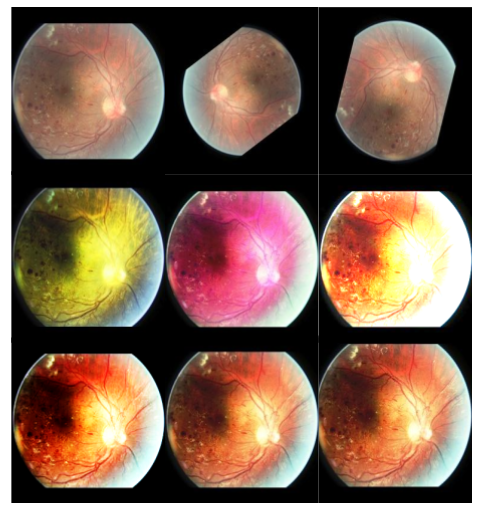
\includegraphics[width=0.4\textwidth]{thumbnail.png}
\caption{Different versions of sample image after augmentation}
\label{example}
\end{figure}

\begin{figure*}
\centering
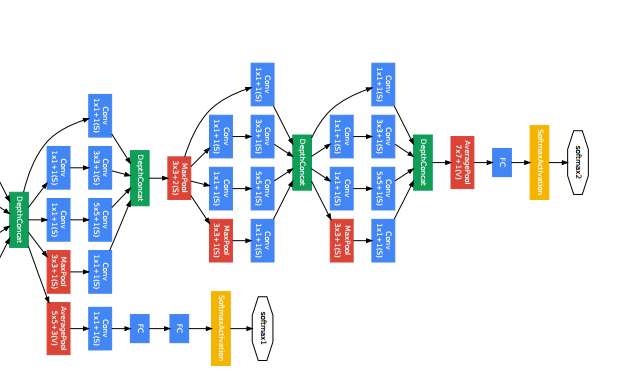
\includegraphics[width=0.8\textwidth]{googlenet_arch.png}
\caption{An overview of GoogLeNet architecture. We include only a portion of the architecture ; please refer to the paper for full architecture.}
\label{googlenet_arch}
\end{figure*}

In our experiments, we examine the performances of different ML models on detecting the severity level of DR (ranging from 0 - 4, where 0 stands for healthy and 4 stands for the most severe DR ). We start with image preprocessing to generate an augmented dataset using different augmentation methods. An example of different versions of selected image is shown in \figref{example}, with more details given in the later section. Then, we use conventional ML techniques to train on a combination of well-craft, generic features that have been demonstrated to be effective in previous studies, for example, the Histogram of Oriented Gradients~(HOG) and Local Binary Patterns~(LBP)~\cite{hog,lbp}. Finally, we explore the effectiveness of some CNN models such as GoogleNet and AlexNet~\cite{GoogleNet,AlexNet}. 

\textbf{Summary of observations.} We find that: 
\begin{itemize}
\item The weighted average accuracy of traditional ML methods with generic features are only slightly better than random-guess. The accuracy of the best-performing classifier is only about 29\%.
\item Without the need of feature selection and parameter tuning, GoogleNet and AlexNet can easily achieve an accuracy above 90\%. The results suggest some advanced CNN networks are very powerful at feature extraction and image classification. 
\end{itemize}

Our paper is organized in the following manner: In the background 
section we introduce the related work on DR detection using 
traditional ML methods and using CNN separately. Then, we describe the dataset we use and how we perform data augmentation. Finally, we explain the experimental 
design, and provide an evaluation of results for traditional ML methods and CNNs respectively. 




\section{Background}
\subsection{Related Work}
Many studies have been conducted on DR classification.\\
\cite{1} used Random Forests to find the impact of sample size on classifier performance and the possibility of using Random forest generated class conditional probabilities as metrics describing DR risk. They find that RF based models produce much higher classification accuracy than those based on logistic regression. Combining both types of data did not increase accuracy but did increase statistical discrimination of healthy participants who subsequently did or did not have DR events during four years of follow-up.

\cite{2} aims to develop an automated screening system to analyze digital color retinal images for important features of non-proliferative diabetic retinopathy. They draw the conclusion that fully automated computer algorithms were able to detect hard exudates and HMA. This provides an inspiration of feature extraction about this topic.

Then, in \cite{3}, the authors develop a system to automatically detect features of DR in color digital retinal images and evaluate the potential of those features in DR screening. They draw the conclusion that at 94.8$\%$ 
With the development of deep learning techniques, some papers have applied several deep-learning models to tackle with this problem. Specifically, convolutional neural networks have been applied for automated, quick and precise identification of the disease.

Authors have previously applyed deep learning techniques to improve the accuracy as well as sensitivity of this problem.

For instance, \cite{4} compares the performance of an automated deep learning algorithm compare with manual grading by ophthalmologists for identifying DR. They train a CNN using a retrospective development data set of 128175 retinal images, which were graded 3 to 7 times for diabetic retinopathy, diabetic macular edema, and image gradability by a panel of 54 US licensed ophthalmologists. It found that in 2 validation sets of 9963 images and 1748 images separately, the algorithm performed well in both high sensitivity and high specificity settings.

Another paper,\cite{5}, compares the performance of a deep-learning enhanced algorithm for automated detection of DR, with a different criteria. They use the previously reported consensus reference standard of referable DR, and calculated negative predictive value, area under the curve and confidence intervals to evaluate the model. They find that a deep-learning enhanced algorithm for this problem will achieve significantly better performance than previously reported while using traditional machine learning techniques. In our paper, we add to the growing base of knowledge of deep learning methods in medical imaging.


Prior works usually only focus on using retina-specific features, such as diameter of optic disk, microaneurysms, and exudates with ML. They do not use consist datasets, evaluation metrics, or 
experiment procedures so it's hard to directly compare the efficiency of their methodologies. Besides, 
the CNN models that have been used are rather ad-hoc. In contrast, we use a consistent dataset and generic, context-independent features for traditional MLs and standard CNN models. We use accuracy as the evaluation metric, which is straightforward and easy-to-understand. Our experiments can better reflect the \emph{portability} of certain features and models, that is, to what extent techniques designed for specific tasks can be applied to broader scenarios. 

\subsection{Convolutional Neural Networks}

As we know, Convolutional Neural Networks (CNNs) have gained remarkable success in computer vision, which is mostly owe to their ability that enables learning rich image representations from large-scale annotated data. In the field of medical image analysis, large amounts if annotated data may be not always available. The number of acquired ground-truth data is sometimes insufficient to train the CNNs without over-fitting and convergence issues from scratch. Hence application of the deep CNNs is a challenge in medical imaging domain.

Several CNN models are used to tackle with this setting in this paper: 

\subsubsection{LeNet}
LeNet is a type of convolutional neural network that is used to recognize patterns from visual images directly without too much preprocessing. Like most of other neural networks, LeNet adopts the back-propagation algorithm to optimize the parameters and the structure of the neural network, while using convolution layers to capture patterns of different scales\cite{LeNet}.

\subsubsection{AlexNet}
AlexNet is another type of convolutional neural network. AlexNet has eight layers, where the first five are convolutional layers and the last three are fully connected layers. There are also pooling and activation process in between the eight layers to group the pooled information together. Compared to LeNet, AlexNet can learn patterns that are not so visually obvious\cite{AlexNet}.

\subsubsection{Network in Network}
Network in Network was developed based on the traditional CNN and made a break through by inventing the inception architecture. It introduces two new concepts: Multi Linear Perceptions Convolution (MLPconv) and Global Average Pooling (GAP). MLPconv is the idea to replace linear filters with filters with different sizes within the receipt field, which allow better feature extraction and higher accuracy. GAP means to create as many activation maps as the classes there at the last layer and average the maps to get the final results. These two ideas reduce parameter numbers and computation complexity significantly \cite{nin}.

\subsubsection{GoogLeNet}
Inspired by Network in Network, GoogLeNet is a 22 layers deep neural network that utilize 9 inception module, where each module convolves using filters with different sizes that captures both the most accurate details and large scale information of the data. Therefore, GoogLeNet is able to utilize the information more efficiently by covering a larger amount of data while training, but also keep the computational cost at the same level with traditional convolutional neural network.  GoogleNet has less parameters than AlexNet and performs faster and much more accurate\cite{GoogleNet}.





\section{Dataset}

The original dataset is provided by EyePACS and can be downloaded from \url{https://www.kaggle.com/c/diabetic-retinopathy-detection/data}. The dataset contains a total of 35,126 labeled RGB images. The image labels indicate the severity level of DR,  which is encoded as 0, 1, 2, 3, and 4, corresponding to \texttt{No DR}, \texttt{Mild DR}, \texttt{Moderate DR}, \texttt{Severe DR},  and \texttt{Proliferative DR}. The distribution of different class of images are show in \tabref{cls_dist}.

\begin{table}[t]
\centering
\scriptsize
\begin{tabular}{|r|r|r|r|r|r|}
\hline
Class label & \begin{tabular}[c]{@{}r@{}}0 \\ (No DR)\end{tabular} & \begin{tabular}[c]{@{}r@{}}1 \\ (Mild)\end{tabular} & \begin{tabular}[c]{@{}r@{}}2 \\ (Moderate)\end{tabular} & \begin{tabular}[c]{@{}r@{}}3 \\ (Severe)\end{tabular} & \begin{tabular}[c]{@{}r@{}}4 \\ (Proliferative)\end{tabular} \\ \hline
Image No. & 25810 & 2443 & 5292 & 873 & 708 \\ \hline
\end{tabular}
\caption{The class distribution of EyePACS retinal image dataset}
\label{cls_dist}
\end{table}

We firstly drew 500 images from each class randomly, and then performed offline data augmentation. We adopted the following image transformation methods for data augmentation: stretch image, random image rotation, and adjustment of contrast level, hue level and brightness. Given the limited computing resources we have, we performed all the data augmentation against the original sampled images instead of chaining the methods. More specifically, we stretched the image using a ratio that was randomly selected from range 0.8 - 1.5~ (augmentation factor x1), rotated an image by 18 different angles (x18), adjusted the image to two different contrast levels (x2), hue levels (x2), and brightness levels (x2). As a result, we got a total of 65,000 images (including the original images).Then we split the image into train(80\%) and test(20\%) dataset. The validation sets which take 10\% of the train dataset were be randomly selected during model selection.  After augmentation, we resized all the images to 256x256x3 for further use. A example of different versions of a given image is shown in \figref{example}. Note that for CNN training, we also performed on-the-fly data augmentation using the methods supported by the framework we used (Caffe~\cite{jia2014caffe}), which are: mirror and random crop. This could further increase the size of our dataset. 


\section{Traditional Machine Learning}

\subsection{Feature Generation}

To extract features, we firstly converted all images to grayscale. Then, we 
considered the following image features:


% \begin{figure}[t]
% \centering

% \caption{Confusion matrix for binary-classification }
% \label{cmbin}
% \end{figure}

We showed the changes of the average training accuracy under different numbers of PCA 
components in \figref{pcamulti} in both settings. 




\begin{figure}[t]
\centering
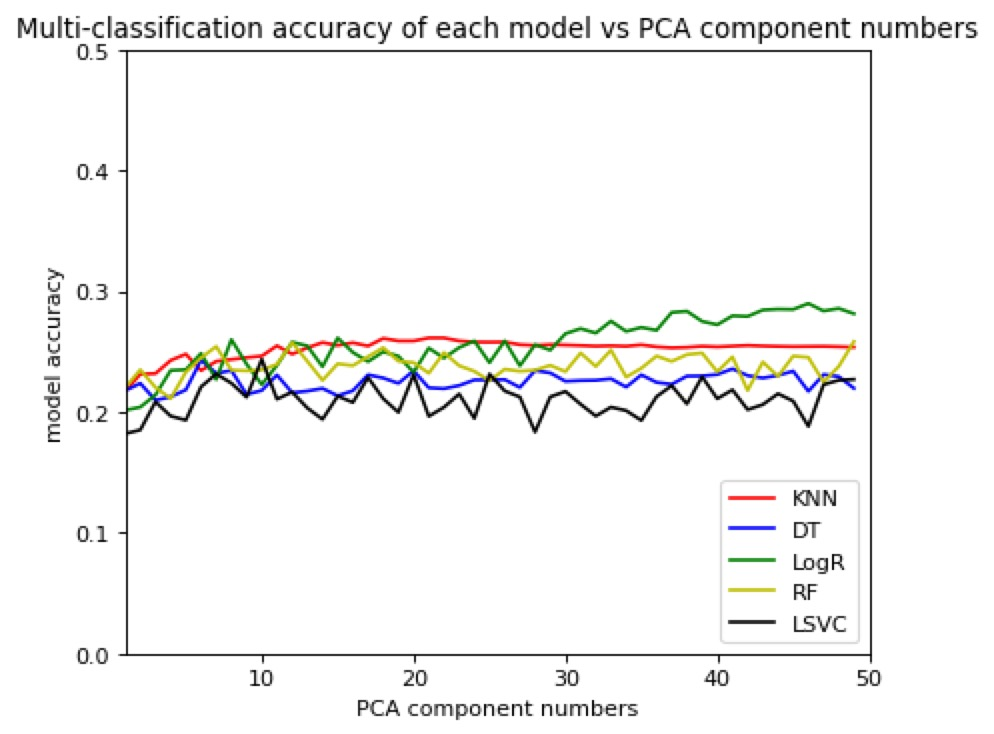
\includegraphics[width=0.4\textwidth]{multi_class.jpeg}
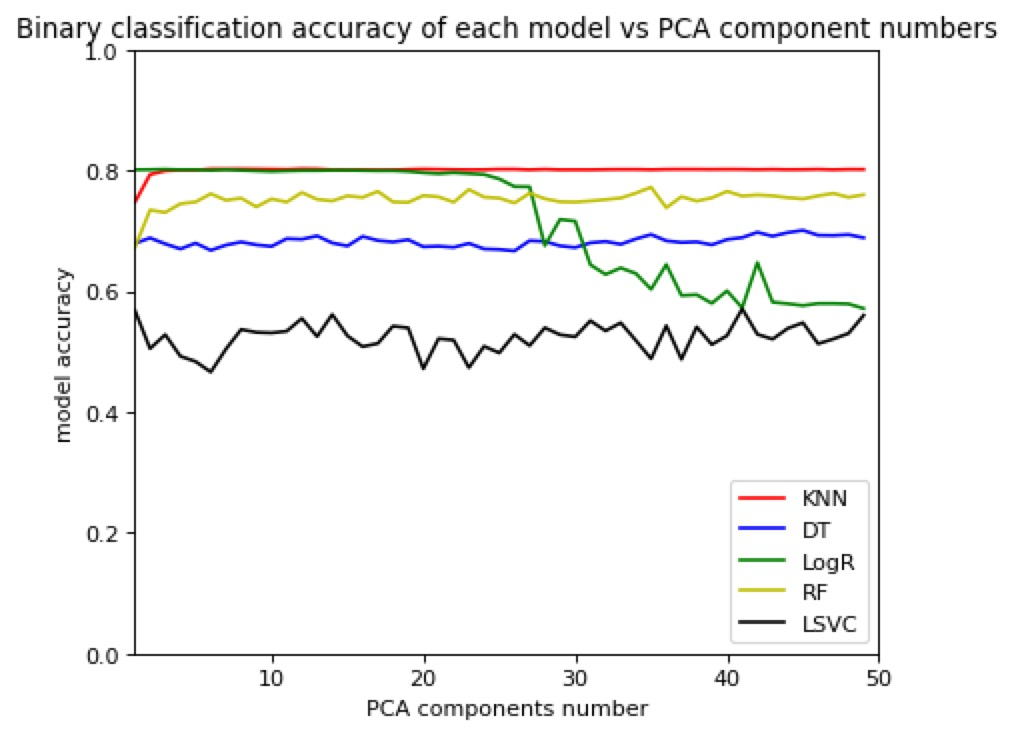
\includegraphics[width=0.4\textwidth]{binrary_class.jpeg}
\caption{Training accuracy of selected models vs. PCA component numbers in 
multi-classification (left) and binary-classification (right)}
\label{pcamulti}
\end{figure}
% \begin{figure}[t]
% \centering
% 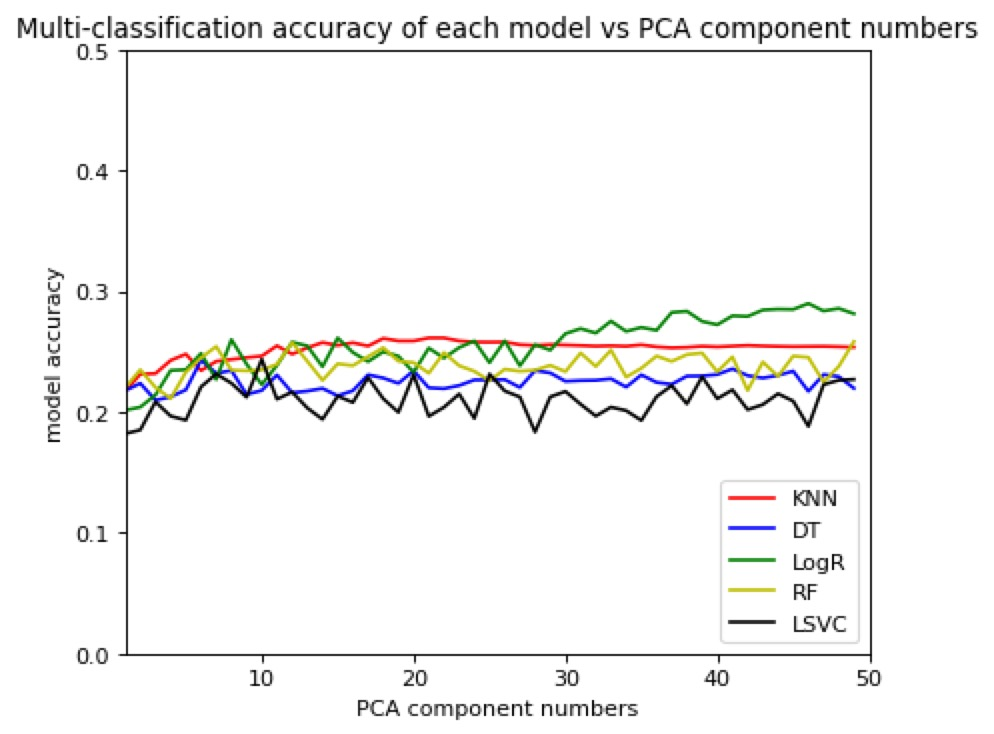
\includegraphics[width=0.4\textwidth]{multi_class.jpeg}
% \caption{Multi-classification accuracy of each model vs PCA component numbers}
% \label{pcamulti}
% \end{figure}

% \begin{figure}[t]
% \centering
% 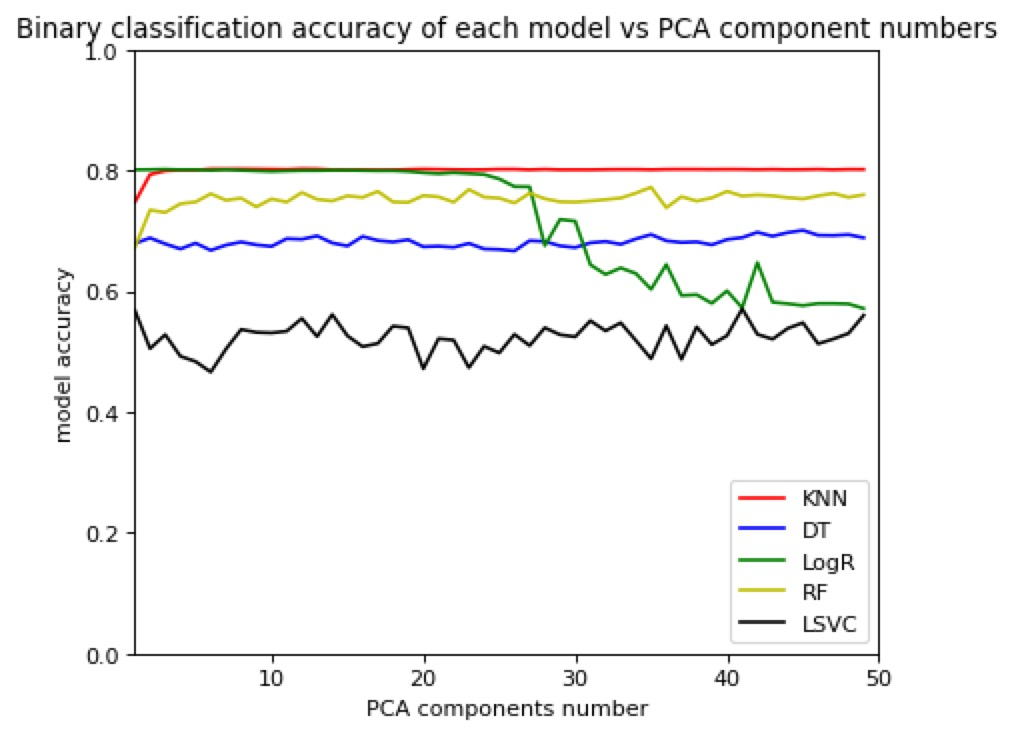
\includegraphics[width=0.4\textwidth]{binrary_class.jpeg}
% \caption{Binary-classification accuracy of each model vs PCA component numbers}
% \label{pcabin}
% \end{figure}

\begin{itemize}
\item Histogram of Pixels (HP): the distribution of pixel values (i.e., the number of pixels of the same value), which resulted in 256-dimension feature vector. 
\item Histogram of oriented gradients (HOG): used to detect the object. It counts occurrences of gradient orientation in localized portions of an image. This method produced a 64-dimension feature vector~\cite{hog}.
\item Haralick Texture (HAK): a feature matrix that counts the co-occurrence of neighboring gray levels in the image. It is used to quantify an image based on texture. This matrix has the dimension of gray levels N in the region of interest (ROI). We generated a 13-dimension feature vector using this method~\cite{haralick}.
\item Local Binary Patterns (LBP): summarizes the local structure in an image by comparing each pixel with its neighborhood. If the intensity of the center pixel is greater or equal to its neighbor, then denote it with 1 and vice versa. This method results in a 20-dimension features vector~\cite{lbp}. 
\item Parameter-Free Threshold Adjacency Statistics (PFTAS): the distribution of white pixels that have zero to N neighbors. In this project, we used the built-in python library Mahotas to build a 54-dimensional PFTAS-feature vector~\cite{pftas}.
\item Image moments: the weighted average of the image pixels intensity. It is useful for catching image properties. 
We applied two different ways, Zernike Moments (ZM) and Hu moments (HU), to obtain a 32-dimension feature vector~\cite{zm,hu}.
\item Scale-Invariant Feature Transform (SIFT): SIFT is an algorithm for detecting and describing 
local features in images. We generated a 2,048-dimension feature vector using it~\cite{sift}. 	
\end{itemize}

All features have been shown to be sufficient under various settings in the image classification tasks. Note that the standard way to identify diabetic retinopathy 
severity level is to examine the blood vessels, microaneurysms, and exudates in 
the retina~\cite{1,2,3}. Our goal is to use those image recognition and objection detection algorithms  
to catch these characteristics of retina. We finally extract 2,497 features from for each image. In the next session we performed 
feature dimension reduction to filter out important features from the 2497 features. 	

\begin{figure}[t]
\centering
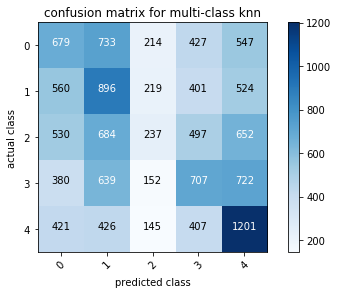
\includegraphics[width=0.35\textwidth]{multi.png}
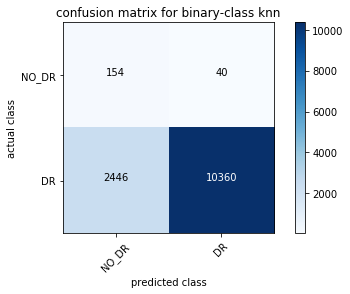
\includegraphics[width=0.35\textwidth]{binary_knn.png}
\caption{Confusion matrices of KNN 
in multi-classification~(left) and logistic regression in binary-classification(right) }
\label{cmmulti}
\end{figure}

\subsection{Model Selection}

The model selection pipeline is as follows: firstly apply PCA to all the features using $m$ as the PCA component number; then, for a given model $m$ and the model parameter $p$, train a classifier on the training set with 10-fold CV, and record the average classification accuracy. That means to explore every possible combinations of ($n$, $m$, $p$), and select the setting that produce the highest accuracy. 

The number of PCA components $n$ we have tested ranging from 1 to 50. We considered the following seven conventional ML models: CART decision tree, extra tree, KNN,  SVM, logistic regression, random forest, and AdaBoost with decision tree.  For binary classifiers, we used the one-vs-rest strategy, which is the most commonly used strategy for multiclass classification.  We trained one classifier for each of the classes against all the other classes (i.e., class as positive and all the other classes as negatives), and vote the output that has the highest confidence score as the class for a given test sample. We fixed the parameters being used for most of the models based on the suggestions from Sklearn, except for KNN. For KNN, we varied the number of neighbors from 1 to 30. 

\subsection{Evaluation}
We considered two settings: 
\begin{itemize}
\item Multiclass classification: classify an image based on its severity level 0 -- 4. 
\item Binary classification: label an image as \texttt{NoDR} or \texttt{DR}, with all the images of severity 1 -- 4 been considered as \texttt{DR} and severity 0 as \texttt{NoDR}. Binary classification is more commonly discussed in literatures. 
\end{itemize}

\begin{figure}[t]
\centering
%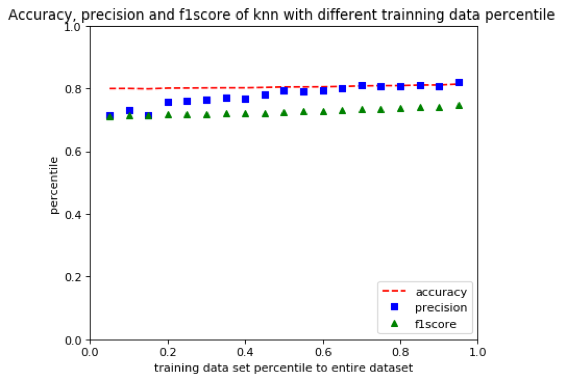
\includegraphics[width=0.4\textwidth]{accuracy.png}
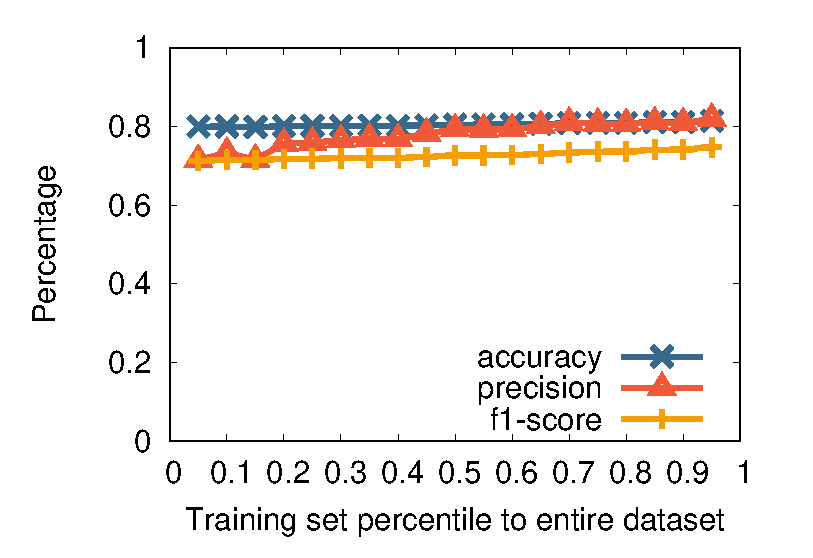
\includegraphics[width=0.4\textwidth]{knn.eps}
\caption{Accuracy, precision and f1-score of KNN with different training data percentile }
\label{knnacc}
\end{figure}


\begin{figure}[t]
\centering
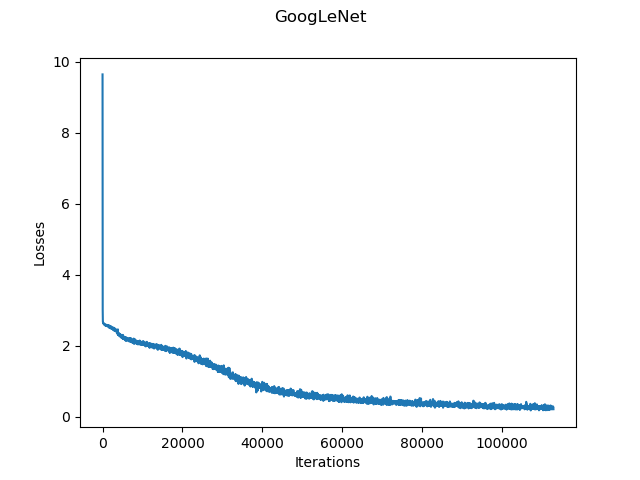
\includegraphics[width=0.35\textwidth]{google_loss.png}
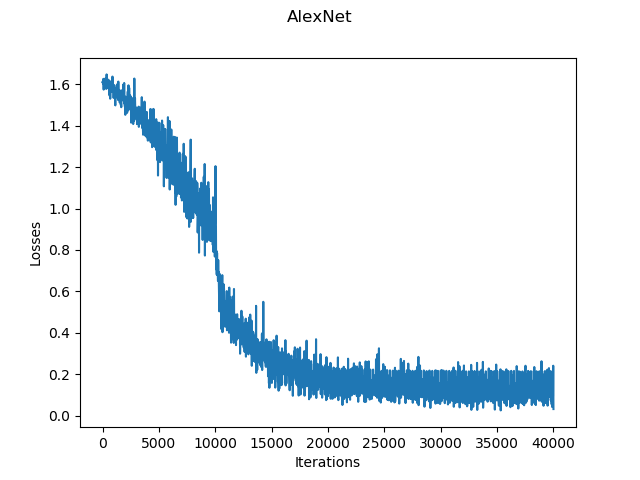
\includegraphics[width=0.35\textwidth]{alex_loss.png}
\caption{Loss vs. iteration numbers for GoogLeNet and AlexNet}
\label{cnn_loss}
\end{figure}

\subsubsection{Multiclass setting}
The logistic regression model produced the highest accuracy, 28.98\%, when $n = 46$. Unfortunately, none of the models produced more than 30\% accuracy. We then repeated the model selection procedures multiple times and see consistent results:  logistic regression with $n = 45$ or $n = 46$ gives 
the highest accuracy $\approx$ 30\%. 

We applied this best model to the test dataset and the resulting accuracy is 28.62\%. This is 
just slightly better than random guessing for 5-class classification. 
The confusion matrix is shown in \figref{cmmulti}. 

\subsubsection{Binary setting}
In binary setting, KNN with 22 neighborers produced the highest accuracy when 
$n = 20$, and the corresponding accuracy on test set is 80.19\%. The confusion matrix is shown in \figref{cmmulti}. For comparison, 
we also tested the other models against the test set, and found indeed the selected 
KNN model gave the best performance: the other models only have 50\% to 78\% 
accuracy on the test set. Surprisingly, SVM with non-linear kernels, which is 
the default choice and has been considered as one of the most effective setting in many prior image 
classification works, perform poorly this time,even worsen than SVM with linear kernels. 

We further examined how would the test accuracy 
changes under different train/test set splits with fixed parameter settings. As shown in \figref{knnacc} 
the weighted test accuracy, precision, and f1-score increases as the training set 
size increases. However, even using a small training dataset, KNN still produces a 
more than 70\% accuracy on testing dataset, which is much better than the best accuracy 
SVM can achieve.  

We show how training accuracy changes under different PCA component numbers in~\figref{pcamulti}. The series represent different machine learning 
algorithms. For a given algorithm, we fixed the parameters as the best-performing 
ones among all testings. As we can see, the accuracy for most algorithms 
are almost the same as the number of PCA components increases. The training 
accuracy of logistic regression are comparable to KNN when PCA component 
number $<$ 25, but decreased quickly as PCA component number went up. 
We didn't test larger PCA component numbers as doing so might be conflict with the idea of dimension reduction. 
One idea is to use deep neural networks to generate more representative features 
as the inputs to our machine learning classifiers. We would like to examine 
this idea in the future.

\section{Discussion}
Our experiments suggest the traditional machine learning models perform poorly 
for identifying the severity level based on retina images, using generic image 
features. However, to simply diagnose if a person has DR or not, the traditional 
models work, and have relatively better accuracy. Unfortunately, the performance 
of our models are still worsen than some of the prior works~\cite{1,2,3}, which used ML with  
retina-specific features, such as diameter of optic disk, microaneurysms, 
and exudates. Nevertheless, our results indicate that ML with  
generic images features are capable, to some extent, to catch 
characteristics of domain-specific images. 







\section{Convolutional Neural Networks}


\begin{table}[t]
\centering
\begin{tabular}{|l|l|l|l|}
\hline
 & Top-1 & Top-2 & Top-3 \\ \hline
LeNet & 0.20 &  0.40 & 0.60 \\ \hline
GoogleNet &  0.90 & 0.95 & 0.98 \\ \hline
AlexNet &  0.92 & 0.96 & 0.98 \\ \hline
NiN &  0.29 & - & - \\ \hline
\end{tabular}
\caption{The test top-N accuracies of different CNN networks. For LeNet we reported the best accuracy only for comparison purposes due to failing of convergence.}
\label{CNN_test_accuracies}
\end{table}

\begin{table}[t]
\centering
\scriptsize
\begin{tabular}{|l|l|l|l|}
\hline
Layer & Name & Size & Description \\ \hline
0 & INPUT & 227x227x3 & Size 227x227 with 3 channels \\ \hline
1 & CONV1-96 & 55x55x96 & 11x11 filters at stride 4 \\ \hline
2 & MAX POOL & 27x27x96 & 3x3 filters at stride 2 \\ \hline
3 & NORM & 27x27x96 & Normalization \\ \hline
4 & CONV2-256 & 27x27x256 & 5x5 filters at stride 1 \\ \hline
5 & MAX POOL & 13x13x256 & 3x3 filters at stride 2 \\ \hline
6 & NORM & 13x13x256 & Normalization \\ \hline
7 & CONV-384 & 13x13x384 & 384 3x3 filters at stride 1 \\ \hline
8 & CONV-384 & 13x13x384 & 384 3x3 filters at stride 1 \\ \hline
9 & CONV-256 & 13x13x256 & 256 3x3 filters at stride 1 \\ \hline
10 & MAX POOL & 6x6x256 & 3x3 filters at stride 2 \\ \hline
11 & FC6 & 4096 & Fully Connected layer\\ \hline
12 & FC7 & 4096 &  Fully Connected layer \\ \hline
13 & FC8 & \textbf{5} & class numbers \\ \hline
\end{tabular}
\caption{ AlexNet architecture and parameters}
\label{alexnetstructure}
\end{table}

\begin{figure}[t]
\centering
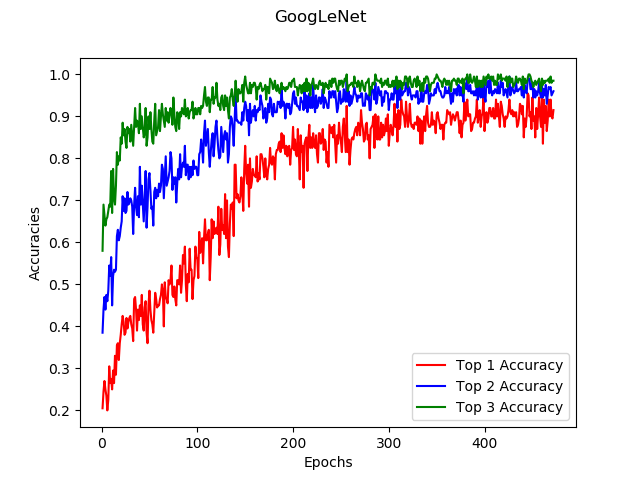
\includegraphics[width=0.4\textwidth]{google_acc.png}
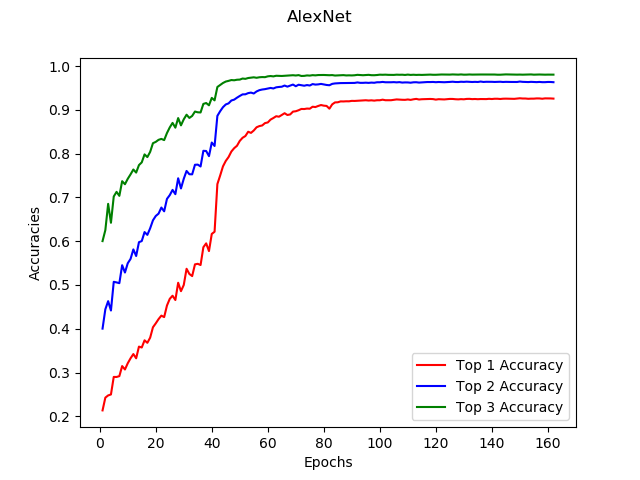
\includegraphics[width=0.4\textwidth]{alex_acc.png}
\caption{Test accuracy vs. epoch numbers for GoogLeNet and AlexNet }
\label{cnn_acc}
\end{figure}

\subsection{Methodology}

We applied different CNN architectures to train 
classifiers from the raw pixels of the images. That is, we transformed  
an image into a 256x256x3 matrix first, where each item in the matrix corresponds 
to a RGB value (without normalization). The classifier took the matrix as input and performed random cropping to fit the input size, 
and further performed predefined data augmentation methods on the matrix. 

We trained four deep models: AlexNet, GoogLeNet, LeNet and Network in Network~(NIN)~
\cite{nin,GoogleNet,LeNet,AlexNet}.
All the parameters were taken from the original papers, except that
we changed the output unit of the networks to 5, corresponding to five classes 
in our case. We showed the structure and parameters we used in AlexNet in \tabref{alexnetstructure}. 
To save space we omitted the parameters of the other models. 

We used Caffe to implement our models. The metrics we considered are training loss 
and test top-N accuracy (N=1,2,3). For top-N accuracy, 
if the target label is in the model's top N predictions with the highest probabilities, 
we consider it as ``correct'', and use the total number of correct classification 
divided by the number of test instances as the top-N accuracy score. 

We fixed the batch size in the training as 200, so it will take 250 iterations to 
complete one epoch. For GoogLeNet, AlexNet and NIN, we set the stepsize to 100,000 (i.e., dropping 
the learning rate every 100\,K iterations) and the momentum to 0.9. The initial 
learning rates are all set to 0.01. We recorded the training loss and test accuracies 
every epoch to examine their trends. 

\begin{figure}[t]
\centering
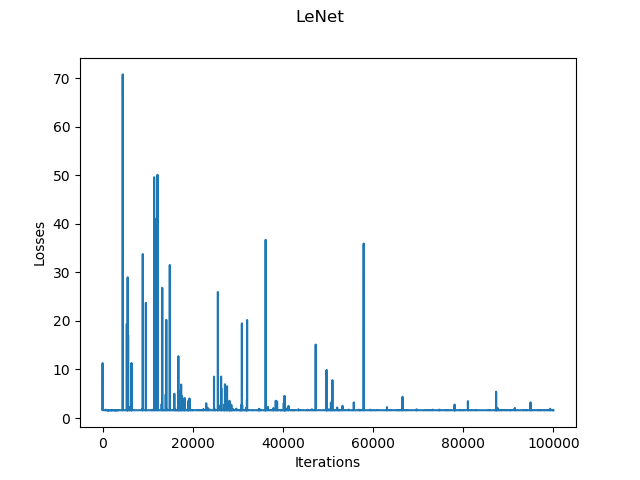
\includegraphics[width=0.4\textwidth]{lenet_loss.png}
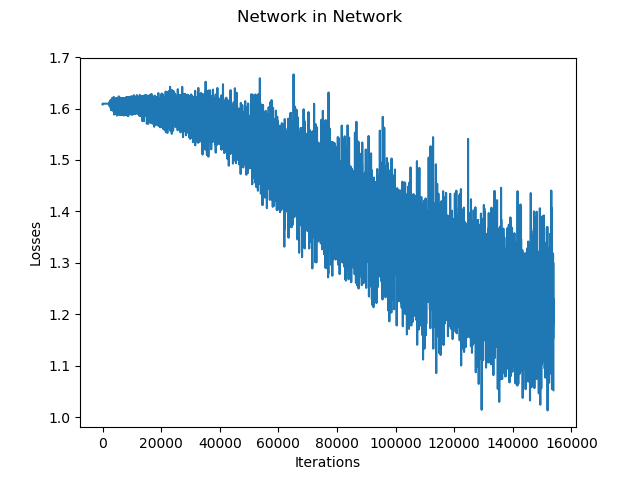
\includegraphics[width=0.4\textwidth]{nin_loss.png}
\caption{Some failures: Loss vs. Iteration for LeNet and Network in Network}
\label{failed_losses}
\end{figure}

\subsection{Evaluation}
A summary of the results can be seen at \tabref{CNN_test_accuracies}. 
On training GoogLeNet and AlexNet, we observe excellent results. For training GoogLeNet, we performed around 120,000 iterations, . We trained AlexNet for 40,000 iterations at a stepsize of 10,000 and the same momentum of 0.9. Compared to the 50-75\% accuracies achieved in the traditional methods, we were able to train our deep NN models of over 90\% accuracy without too much preprocessing (see \figref{cnn_acc}). We note the relative ease with which we could train AlexNet. It took AlexNet only a little more than 20,000 iterations to converge, whereas GoogLeNet required more than 80,000 iterations to achieve similar accuracy (see \figref{cnn_loss}). AlexNet trained faster than an hour using an nVidia GeForce GTX 1080 Titan, whereas GoogNet took us about half a day to fully converge. We count this remarkable behavior toward the simplicity of AlexNet (see \figref{alexnetstructure}), as opposed to the complex inception layout of GoogLeNet (see \figref{googlenet_arch}). 

However, on the other side, we found that CNNs are not a panacea. While testing LeNet and NIN models, we found that both networks fail to converge readily (see \figref{failed_losses}). We did not dig much into why these networks won't work. One possibility for LeNet' failure is that the images are resized to 32x32x3 by the model to cope with its 
input restrictions, therefore many useful information were lost during this processing stage. 
    
\subsection{Discussion}

The simplicity of the machine learning process is obvious when using Deep Convolutional Neural Networks. It allow us to ignore the laborious manual work involved in traditional machine learning methodology such as feature extraction while getting radically better performance. Surprisingly, 
even with relatively small training set (50,000+ images), GoogLeNet and AlexNet can still  
extract high-quality, representative features that can be used to distinguish different classes of images. Our results also show some CNNs might have very good portability and can be even used for domain-specific image~(e.g, medical images) 
classification tasks, as opposed to the suspicions that CNNs are tuned for certain datasets. 





\section{Conclusion}
In our project, we conducted a preliminary examination of performance of traditional machine learning models and standard Convolutional Neural Networks on detecting the severity level of diabetic retinopathy using the color fundus photographs of eyes. While using traditional machine learning methods with well-craft, generic features 
suggested by prior research fail to achieve high accuracies, standard CNN models, GoogleNet and AlexNet, can easily get more than 90\% accuracies with little efforts on feature extraction and parameter tuning. 

Our current implementation treats the CNN model as black box and haven't 
optimized the parameters for our task. For future work, we would like to explore the 
features extracted by CNNs and try to use them as inputs to traditional machine 
learning models. Besides, we would like to examine different ways 
to improve accuracy, for instance, customizing standard CNN models, developing
new CNN models, and assembling different CNN models. Another direction is to 
examine the performance of transfer learning -- using neural network weights from tasks which are related to the specific medical imaging task or other tasks (ImageNet, etc.) to initialize a given CNN model and test against our dataset. 
The motivation for this is that some works have demonstrated that pre-training models  
on ImageNet can be used for classification of x-ray images.  


\bibliographystyle{aaai}
\bibliography{arts}


\end{document}
